%!TEX root = volumeFinal.tex 
\chapter{\label{chap:busca}Busca}

Com o intuito de encontrar uma sequência de ações que um agente consiga alcançar o seu objetivo, é possível utilizar técnicas de busca.
O princípio da busca é encontrar uma solução de um problema através de um conjunto de ações que alcancem o objetivo desejado. 
Para utilizar as técnicas de busca é preciso formalizar o problema a ser resolvido e o objetivo a ser alcançado, pois na busca, como entrada é recebido um problema e é retornado uma solução na forma do conjunto de ações \cite{intelligence2003modern}. 

Um problema pode ser definido por cinco componentes \cite{intelligence2003modern}: \frm[color=yellow]{Refaça as enumerações no estilo que eu fiz no cap anterior.}

\begin{itemize}
	\item $s_{0}$, o estado inicial, que o agente começa no ambiente;
	\item ações, conjunto das possíveis ações presentes no agente;
	\item $resultado(s, a)$, um modelo de transição, que define o estado resultante após a execução da ação a no estado s;
	\item $objetivo(s)$, verifica se o estado é o objetivo do agente; e
	\item custo do caminho, uma função que defina um valor numérico para cada ação realizada em um estado. Essa função pode ser denotada por $c(s, a, s')$, onde s é o estado atual do agente, a é a ação que será aplicada ao estado s e $s'$ é o estado resultante aplicando o modelo de transição resultado(s, a). 
\end{itemize}   


Esses elementos são necessários como entrada para que as técnicas de busca consigam ser utilizadas. As técnicas de busca visam encontrar a solução para esse problema, ou seja, a sequência de ações que leve ao objetivo. 
A solução é obtida quando o agente iniciando no estado inicial do ambiente $s_{0}$, utiliza o modelo de transição $resultado(s, a)$, através das ações aplicadas nos estados, para chegar a um estado onde satisfaça o objetivo do agente $objetivo(s)$.
Existem diferentes técnicas para encontrar uma solução. As diferentes técnicas podem encontrar caminhos diferentes para o mesmo problema, isso vem do fato de que o custo do caminho, quando levado em consideração, pode encontrar uma solução ótima, o que significa que a sequência de ações encontrada é a que tem o menor custo de caminho entre todas as soluções \cite{intelligence2003modern}. \frm[color=yellow]{Não consigo analisar esta frase, \textbf{parse error}}

%Algumas técnicas levam em consideração o custo de cada caminho, para  . 
%Pelo fato de que as técnicas de busca aceitam mais de uma solução para o mesmo objetivo, com conjuntos de ações diferentes, é utilizado para medir a qualidade da solução o custo do caminho, uma solução ótima é tida quando o menor custo do caminho de todas as soluções possíveis é encontrado utilizando o custo do caminho para cada ação realizada \cite{intelligence2003modern}.

Com a finalidade de exemplificar um problema de busca, considere o mapa apresentado na figura \ref{fig:mapabusca}. Cada círculo representa uma cidade, e as linhas entre as cidades são estradas que ligam as cidades uma a outra. A única ação possível é a de se locomover entre as cidades que tenham ligação. O estado inicial é a cidade de São Jerônimo. O resultado do modelo de transição, a cidade resultante após se locomover. O objetivo do agente é chegar na cidade de Porto Alegre e o custo de cada ação é o valor definido em cima de cada transição. \frm[color=yellow]{Parágrafo de uma frase só...}

\begin{figure}[ht]
	\centering
	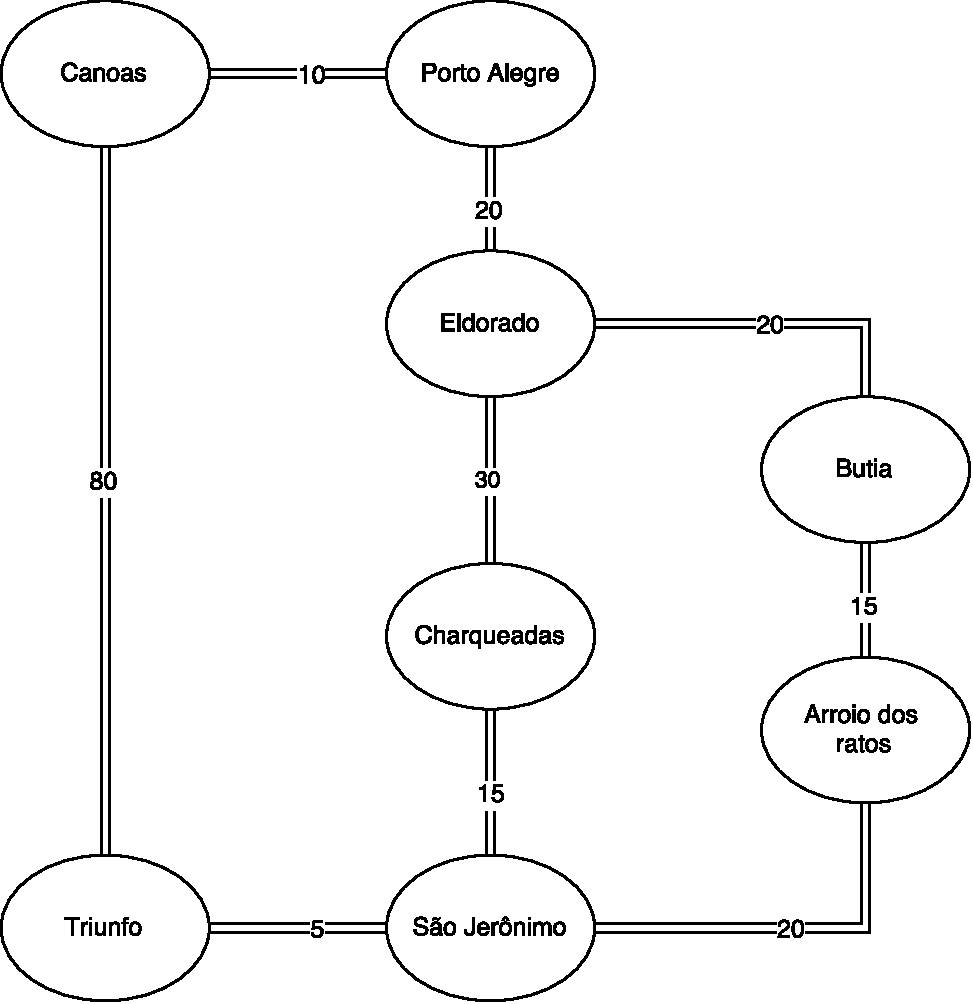
\includegraphics[width=0.6\textwidth]{fig/mapabusca.pdf}
	\caption{Mapa para o exemplo de problema de busca}
	\label{fig:mapabusca}
\end{figure} 

Para atingir o objetivo é preciso tentar os possíveis caminhos até o objetivo. Digamos que o agente comece sua viagem indo para a cidade de Triunfo, para nós, humanos, é intuitivo que a escolha não foi a melhor de início, mas a técnica só terá como saber após realizar todas as possíveis opções de caminhos, ou se utilizar uma técnica que utilize uma função de heurística, levando em consideração os custos dos caminhos, que acrescentam um conhecimento adicional para a resolução do problema \cite{intelligence2003modern}.

\section{Busca adversaria}

Jogos são difíceis de resolver com técnicas de IA, pois eles requerem uma habilidade de tomar algum tipo de decisão, e as técnicas comuns as vezes não são satisfatórias, seja pelo fato dos estados que são possíveis de atingir ser muito grande, ou pelo curto espaço de tempo para tomar a decisão.
A busca adversaria é utilizada nos jogos que estão situados em ambientes competitivos e de multi agentes. Em um jogo o jogador, preferencialmente, não informa suas jogadas previamente, assim tornando o ambiente imprevisível. Os objetivos dos jogadores entram em conflito, pois ambos estão em busca da vitória. 
Com o intuito de resolver esse problema é possível gerar uma solução de contingência para tentar antecipar as jogadas do adversário \cite{intelligence2003modern}. 

As técnicas de busca adversária utilizam uma variação da definição de um problema de busca comum. Os componentes devem se adequar ao ambiente competitivo. Por esse motivo os componentes são redefinidos como:

\begin{itemize}
	\item $s_{0}$, sendo o estado inicial, que especifica como o jogo se configura no início;
	\item $players(s)$, definindo qual jogador tem o movimento no estado $s$;
	\item $actions(s)$, conjunto das ações possíveis em um estado $s$;
	\item $result(s, a)$, um modelo de transição, que define o resultado da ação $a$ a aplicada ao estado $s$;
	\item $terminal(s)$, verifica se o estado $s$ é um estado onde o jogo termina; e
	\item $utility(s,p)$, define um valor numérico, representando o lucro do jogador $p$ ao atingir o estado terminal $s$.
\end{itemize}

Com esses componentes descritos é possível formalizar o que é uma árvore de jogadas. A árvore de jogados ou \textit{game tree} contém os estados do jogo e os movimentos possíveis em cada estado. A \textit{game tree} é composta pelo estado inicial $s_{0}$, as ações $action(s)$ e o modelo de transição $result(s, a)$, e possui uma profundidade $d$, que indica o nível máximo da árvore. 
A árvore representa em cada nodo um estado do jogo e em cada ligação os estados resultantes após a execução de cada ação possível para o estado. Considerando o jogo de jogo da velha, onde cada jogador realiza uma jogada de cada vez, uma \textit{game tree} que mostra parte das jogadas do jogo da velha é ilustrada na Figura~\ref{fig:jogodavelha}. O estado inicial do jogo é o campo vazio, a cada nível da árvore todas as possibilidades de jogadas são testadas, a profundidade $d$ dessa árvore chega a 9 quando ela estiver completa, pois a cada nível da árvore uma jogada é marcada no campo. 

\begin{figure}[ht]
	\centering
	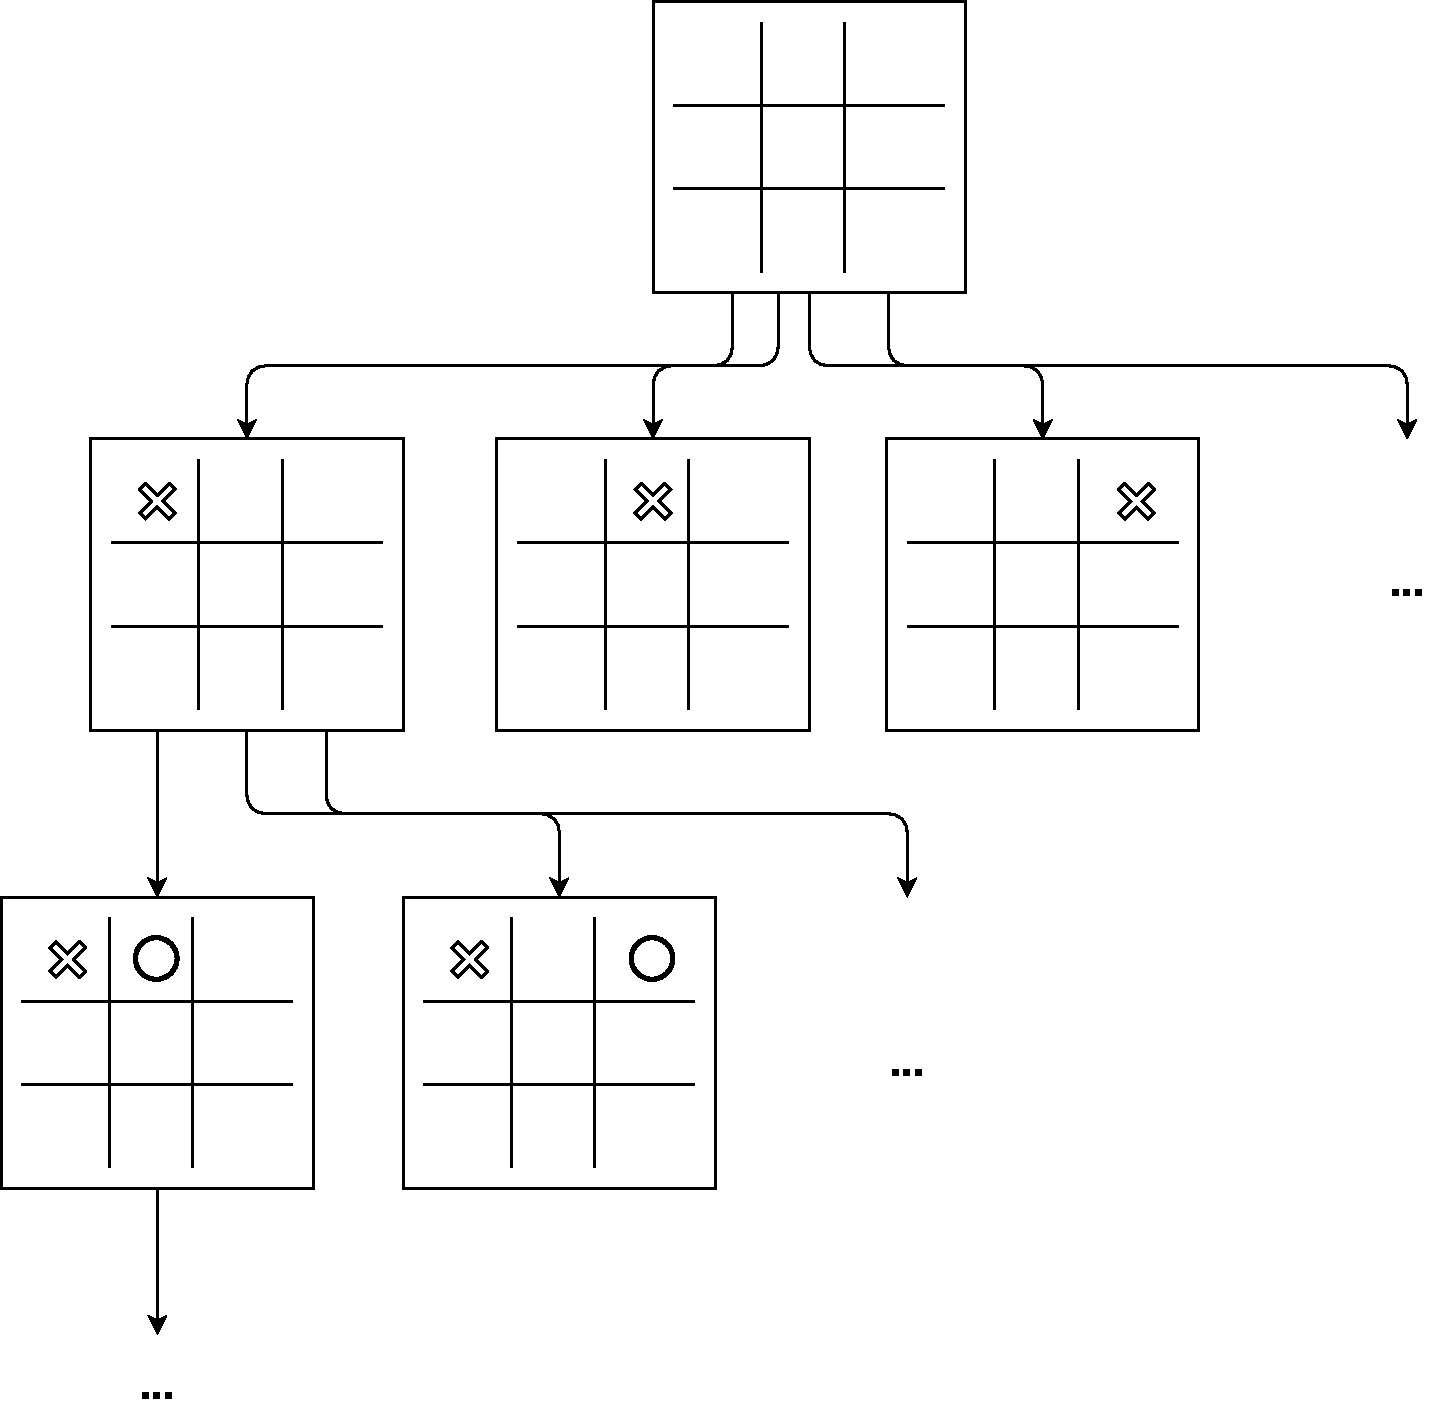
\includegraphics[width=0.5\textwidth]{fig/jogodavelha.pdf}
	\caption{Exemplo de um pedaço de uma \textit{game tree} sobre o jogo da velha}
	\label{fig:jogodavelha}
\end{figure} 

\section{Minimax search}

O algoritmo de \textit{minimax search} é utilizado como uma técnica de busca adversária. O objetivo do algoritmo é retornar a melhor jogada para o estado atual. Esse método considera dois agentes, chamados de \textsc{Max} e \textsc{Min}, onde o jogador \textsc{Max} representa a perspectiva do agente que está tentando maximalizar suas ações em relação ao agente \textsc{Min}, que representa o agente adversário do jogador \textsc{Max}. O algoritmo alterna entre jogadas de \textsc{Max} e \textsc{Min} \cite{intelligence2003modern}. 

O algoritmo utiliza a \textit{game tree} para analisar todos os estados possíveis do jogo, e assim decidir qual a ação que quando aplicada ao seu estado atual, trará um melhor benefício no futuro, se caracterizando a melhor jogada. Os nodos folhas da árvore, que representam o final do jogo, contém um valor de utilidade. Os valores mais altos são as melhores jogadas para \textsc{Max}, e consequentemente, os valores menores são melhores para \textsc{Min}. Ao chegar no final da árvore o algoritmo consegue o valor de utilidade para aquele cenário do jogo, quando isso acontece, o algoritmo faz o caminho inverso na árvore analisando os outros possíveis cenários \cite{intelligence2003modern}. A Figura~\ref{fig:gametree} ilustra esse processo.

\begin{figure}[ht]
	\centering
	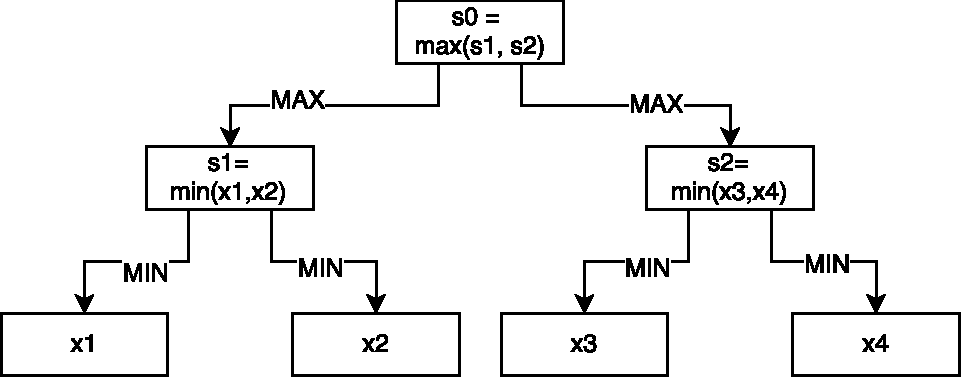
\includegraphics[width=0.6\textwidth]{fig/gametree.pdf}
	\caption{Exemplo de game tree utilizando \textit{minimax search}}
	\label{fig:gametree}
\end{figure} 

O método de \textit{minimax search} assume que os todos os jogadores como sendo racionais, com isso o algoritmo considera que as ações tomadas pelos agentes sempre realizarão uma jogada para tentar ganhar o jogo. O algoritmo de \textit{minimax search} é apresentado no Algoritmo~\ref{alg:minimax}. O algoritmo tem como retorno a melhor ação a ser realizada no estado atual. As funções presentes nas linhas~\ref{alg:minimax:max} e ~\ref{alg:minimax:min} são utilizadas para calcular a jogada na visão de \textsc{Max} e \textsc{Min} respectivamente.
A função presente na linha~\ref{alg:minimax:minimax} é utilizada para iniciar a recursão e ao final retornar o melhor valor de utilidade.

\begin{algorithm}
	\caption{Minimax Search}
	\label{alg:minimax}
	\begin{algorithmic}[1]	
		\Function{Minimax}{$state$} \label{alg:minimax:minimax}
		\State \Return $arg max_{action \in actions(s)} min\_value(result(state, action)) $
		\EndFunction \\
		\Function {Max\_Value}{$state$}\label{alg:minimax:max}
		\If {$terminal(state)$}
		\State	\Return $utility(state)$
		\EndIf
		\State $v = -\infty$
		\ForAll{$action \in actions(state)$}
		\State $v = max(v, min\_value(result(state,action)))$
		\EndFor	
		\EndFunction \\
		\Function {Min\_Value}{$state$}\label{alg:minimax:min}
		\If {$terminal(state)$}
		\State	\Return $utility(state)$
		\EndIf
		\State $v = \infty$
		\ForAll{$action \in actions(state)$}
		\State $v = min(v, max\_value(result(state,action)))$
		\EndFor	
		\EndFunction
	\end{algorithmic}
\end{algorithm}

O algoritmo de \textit{minimax} deve explorar todo o espaço de estados para conseguir encontrar a ação que deve ser executada. A quantidade de estados possíveis, dependendo da situação, pode ser muito alta, no xadrez esse número chega a $10^{50}$, em um jogo de \textit{poker} no estilo \textit{texas holdem} esse número pode chegar a $10^{80}$. Geralmente, as ações devem ser tomadas em uma quantidade de tempo muito pequena. Por esse motivo, utilizar técnicas de busca para jogos pode ser um problema. Existem algumas abordagens que utilizam busca adversaria com um nível de abstração mais alto para tentar minimax esse problema \cite{ontanon2013survey}. \frm[color=yellow]{Finaleira meio rasa de capítulo. Eu esperava algum insight maior disto. Especialmente no tocante a jogos com grandes espaços de estados.} 

